\documentclass[a4paper, 12pt]{article}

% a nice font
\usepackage{kpfonts}

% basic text stuff
\usepackage[utf8]{inputenc}
\usepackage[T1]{fontenc}

\usepackage{tikz} % main tikz package
\usepackage{pgfplots} % for surface plotting

\usetikzlibrary{arrows}

\pgfplotsset{
    compat = 1.17, % to have the same coordinate system between axis and draw
}

% for a nicer colorscheme
\definecolor{blue}{rgb}{0.38, 0.51, 0.71} %glaucous, 97,130,181, #6182B5
\definecolor{darkblue}{RGB}{17, 42, 60} % 112A3C
\definecolor{red}{RGB}{175, 49, 39} % AF3127

\definecolor{orange}{RGB}{217, 156, 55} % D99C37
\definecolor{green}{RGB}{144, 169, 84} % 90A954
\definecolor{palegreen}{RGB}{197, 184, 104} % C5B868

\definecolor{yellow}{RGB}{250, 199, 100} % FAC764
\definecolor{brokenwhite}{RGB}{218, 192, 166} % DAC0A6
\definecolor{brokengrey}{rgb}{0.77, 0.76, 0.82} % {196,194,209}, C4C2D1


\begin{document}
    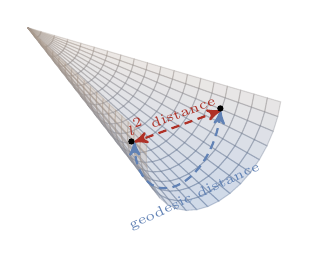
\begin{tikzpicture}[>=stealth']
        \begin{axis}[%
            axis equal,
            width=10cm,
            height=10cm,
            axis lines = center,
            xlabel = {},
            ylabel = {},
            zlabel = {},
            hide axis,
            ticks=none,
            enlargelimits=0.3,
            colormap={whiteblue}{color=(blue) color=(white)},
            colormap={gb}{color=(green) color=(yellow)
                color=(brown)},
            view/h=45,
            scale uniformly strategy=units only,
            declare function = {
                conez(\u,\v) = \u*sin(20)*cos(\v);
                coney(\u,\v) = \u*sin(20)*sin(\v);
                conex(\u,\v) = \u*cos(20);
                vt(\v) = 36 - (\v-270)*(\v-270) / 10000 * 2;
                vtx(\t) = conex(vt(120), 120) + \t * (conex(vt(270), 270) - conex(vt(120),120));
                vty(\t) = coney(vt(120), 120) + \t * (coney(vt(270), 270) - coney(vt(120),120));
                vtz(\t) = conez(vt(120), 120) + \t * (conez(vt(270), 270) - conez(vt(120),120));
            },
        ]
        \addplot3[%
            opacity = 0.3,
            %z buffer = sort,
            surf,
            samples = 20,
            variable = \u,
            variable y = \v,
            domain = 0:40,
            y domain = 100:280,
            colormap={slategraywhite}{rgb255=(97,130,181) rgb255=(218, 192, 166)},
        ]
        ({conex(u,v)}, {coney(u,v)}, {conez(u,v)});

        \addplot3+[%
            samples = 30,
            thick,
            densely dashed,
            variable = \v,
            domain = 120:270,
            no markers,
            samples y = 0,
            color=blue,
            <->,
        ]
        ({conex({vt(v)},v)}, {coney({vt(v)},v)}, {conez({vt(v)},v)});
        %({conex({ut1(u,v)},{vt1(u,v)})},{coney({ut1(u,v)},{vt1(u,v)})},{conez({ut1(u,v)},{vt1(u,v)})});

        \addplot3+[%
            samples = 30,
            variable = \t,
            domain = 0:1,
            thick,
            densely dashed,
            no markers,
            samples y = 0,
            color=red,
            <->,
        ]
        ({vtx(t)}, {vty(t)}, {vtz(t)});


        \end{axis}

        \coordinate (A) at (3.4,2.2);
        \fill (A) circle (0.04);

        \coordinate (B) at (4.53,2.62);
        \fill (B) circle (0.04);

        \coordinate (geo) at (4.2,1.5);
        \node[rotate=25] at (geo) {\color{blue}{\tiny{geodesic distance}}};

        \coordinate (l2) at (3.9,2.55);
        \node[rotate=20] at (l2) {\color{red}{\tiny{$l^2$ distance}}};
               
   \end{tikzpicture}
\end{document}
